% !TEX encoding = UTF-8
%Koma article
\documentclass[fontsize=12pt,paper=letter,twoside]{scrartcl}
\usepackage{float}
\usepackage{listings}

%Standard Pre-amble
\usepackage[top=4cm,bottom=4cm,left=3cm,right=3cm,asymmetric]{geometry}
%\geometry{landscape}                % Activate for for rotated page geometry
%\usepackage[parfill]{parskip}    % Begin paragraphs with an empty line rather than an indent
\usepackage[table,xcdraw]{xcolor}
\usepackage{graphicx}

\usepackage{amsmath}
\usepackage{amssymb}
\usepackage{epstopdf}
\DeclareGraphicsRule{.tif}{png}{.png}{`convert #1 `dirname #1`/`basename #1 .tif`.png}
% Listings needs package courier
\usepackage{listings} % Needs 
\usepackage{courier}

\usepackage[framemethod=TikZ]{mdframed}
\usepackage{url}

\usepackage{sty/bsymb} %% Event-B symbols
\usepackage{sty/eventB} %% REQ and ENV
\usepackage{sty/calculation}

%Maths
\usepackage{amssymb,amsmath}
\def\Fl{\mathbb{F}}
\def\Rl{\mathbb{R}}
\def\Nl{\mathbb{N}}
\def\Bl{\mathbb{B}}
\def\St{\mathbb{S}}
\newcommand{\ovr}{\upharpoonright}
\newcommand{\var}[1]{\textit{#1}}
%Useful definitions
\newcommand{\mv}[1]{\textit{m\_#1}}
\newcommand{\cv}[1]{\textit{c\_#1}}
\newcommand{\degree}[1]{^{\circ}\mathrm{#1}}
%\newcommand{\comment}[1]{{\footnotesize \quad\texttt{--}\textrm{#1}}}
\newcommand{\im}[1]{i\texttt{-\!#1}}

\usepackage[headsepline]{scrpage2}
\pagestyle{scrheadings}
\ihead[]{\small EECS4312 Report1}
\ohead[]{\small \thepage}
\cfoot[]{}
\ofoot[]{}


%%%%PVS environment%%%%%%%%%%%%%%%%%%%
\lstnewenvironment{pvs}[1][]
    {\lstset{#1,captionpos=b,language=pvs,
    mathescape=true,
    basicstyle=\small\ttfamily,
    numbers=none,
    frame=single,
    % numberstyle=\tiny\color{gray},
    % backgroundcolor=\color{lightgray},
    firstnumber=auto
    }}
    {}
 %%%%%%%%%%%%%%%%%%%%%%%%%%%%%%%%
 
%%%%Verbatim environment%%%%%%%%%%%%%%%%%%%
\lstnewenvironment{code}[1][]
    {\lstset{#1,captionpos=b,
    mathescape=true,
    basicstyle=\small\ttfamily,
    numbers=none,
    frame=single,
    % numberstyle=\tiny\color{gray},
    % backgroundcolor=\color{lightgray},
    firstnumber=auto
    }}
    {}

% \newenvironment{boxed}[1]
%    {\begin{center}
%    #1\\[1ex]
%    \begin{tabular}{|p{0.9\textwidth}|}
%    \hline\\
%    }
%    { 
%    \\\\\hline
%    \end{tabular} 
%    \end{center}
%    }
 %%%%%%%%%%%%%%%%%%%%%%%%%%%%%%%%
 
 %Text in a box
\newenvironment{textbox}
    {\begin{center}
    \begin{tabular}{|p{0.9\textwidth}|}
    \hline\\
    }
    { 
    \\\\\hline
    \end{tabular} 
    \end{center}
    }

\usepackage{hyperref}

%Highlight \hl{}
\usepackage{soul}

\usepackage{enumitem}
\newlist{mylist}{itemize}{1}
\setlist[mylist]{label=\textbullet,leftmargin=1cm,nosep}

\usepackage{multirow}

% Reduce space between figure and caption
%\usepackage{caption}
%\captionsetup[table]{font=small,skip=0pt}     %% Adjust here
%or equivalently 
\usepackage[font=small,skip=4pt]{caption}
%Useful definitions
%\newcommand{\mv}[1]{\textit{m\_#1}}
%\newcommand{\cv}[1]{\textit{c\_#1}}
%\newcommand{\degree}[1]{^{\circ}\mathrm{#1}}
%\newcommand{\comment}[1]{{\footnotesize \quad\texttt{--}\textrm{#1}}}

% Set the header
\ihead[]{\small EECS4090 Project}


%%%%%%%%%%%%Enter your names here%%%%%%%%
\author{\textbf{Edward Vaisman}
\and \textbf{Sadman Sakib Hasan}
}
%%%%%%%%%%%%%%%%%%%%%%%%%%%%%%%%

\date{\today} % Display a given date or no date

\begin{document}
\title{Grad Apps 2.0 \\ Admission Committee Member User Manual}
\maketitle

\newpage

%%%%%%%%%%%%%%%%%%%%%%%%%%%%%%%
\tableofcontents

\newpage


%%%%Rest of your document goes here%%%%%%%%%%%%%%%%%%%

\clearpage
\section{User Overview}

The \emph{admission committee member} in our system under description is a subset of EECS graduate program members who are in charge of reviewing new applications. In addition to reviewing an application, an admission committee member can view past reviewed applications and apply filters on them. A breakdown of a \emph{committee member's} permissible actions is listed below.

\smallskip
\noindent A \emph{committee member}:

\begin{mylist}
\item Shall be able to view current and past reviewed application(s).
\item Shall be able to apply filters on current and past reviewed application(s).
\item Shall be able to review an assigned application(s).
\item Shall be able to save a review as a draft for later completion.
\item Shall be able to add new university assessments in the system to be used in a review. Such a new assessment will be added globally to the system and can be seen and used by other committee members when filling out a review.
\end{mylist}

\section{Authentication}

In order for a user to sign in to the application as a committee member, they need to be assigned to the \emph{Committee Member} role by the system administrator. Once the user has been granted access to the role, they can sign in to the system and select the \emph{Committee Member} role.

\begin{figure}[!htb]
\begin{center}
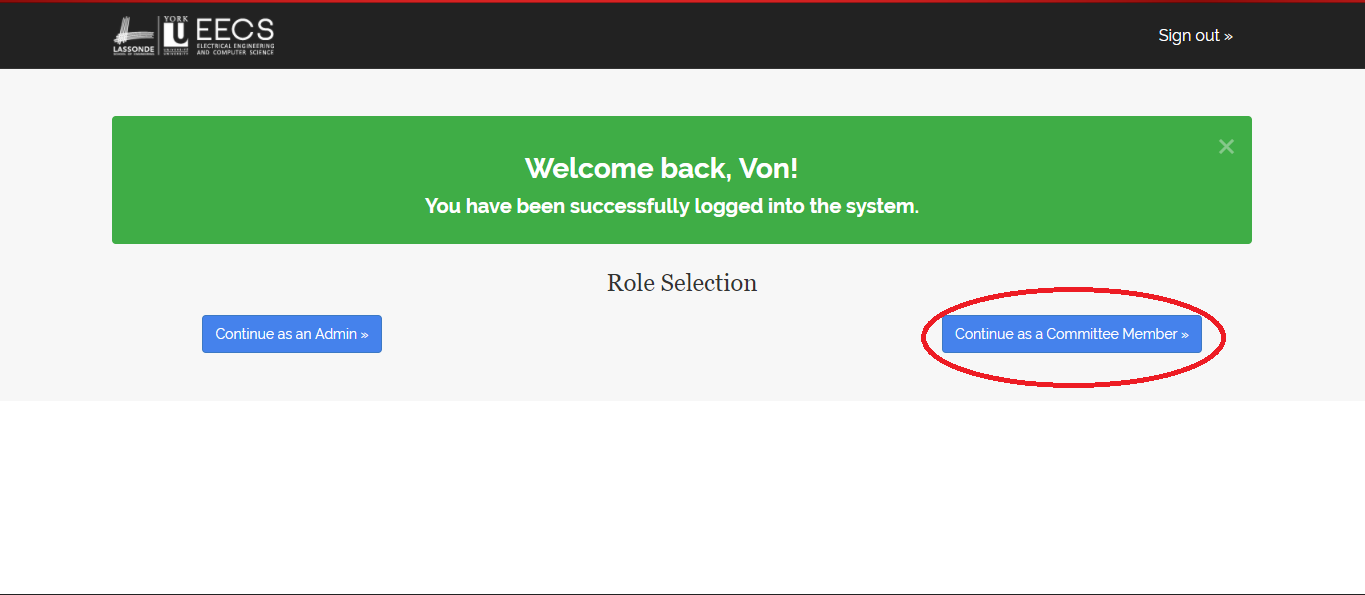
\includegraphics[width=.9\textwidth]{images/auth.png}
\end{center}
\caption{Select Committee Member Role}
\label{fig:role_selection}
\end{figure}

\bigskip
\noindent \textbf{Note:} Once the user has been authenticated, the system automatically signs the user out after 15 minutes of inactivity within the application. This is to ensure the security of the overall system to protect both student confidential data and logged in user data.


\section{Committee Member Portal}

After the user has signed in to the system and selected the \emph{Committee Member} role, they shall be redirected to the committee member portal. The portal by default shows all past and current reviewed applications assigned to the logged in user for the current study year ordered by the date assigned in ascending order.

\begin{figure}[!htb]
\begin{center}
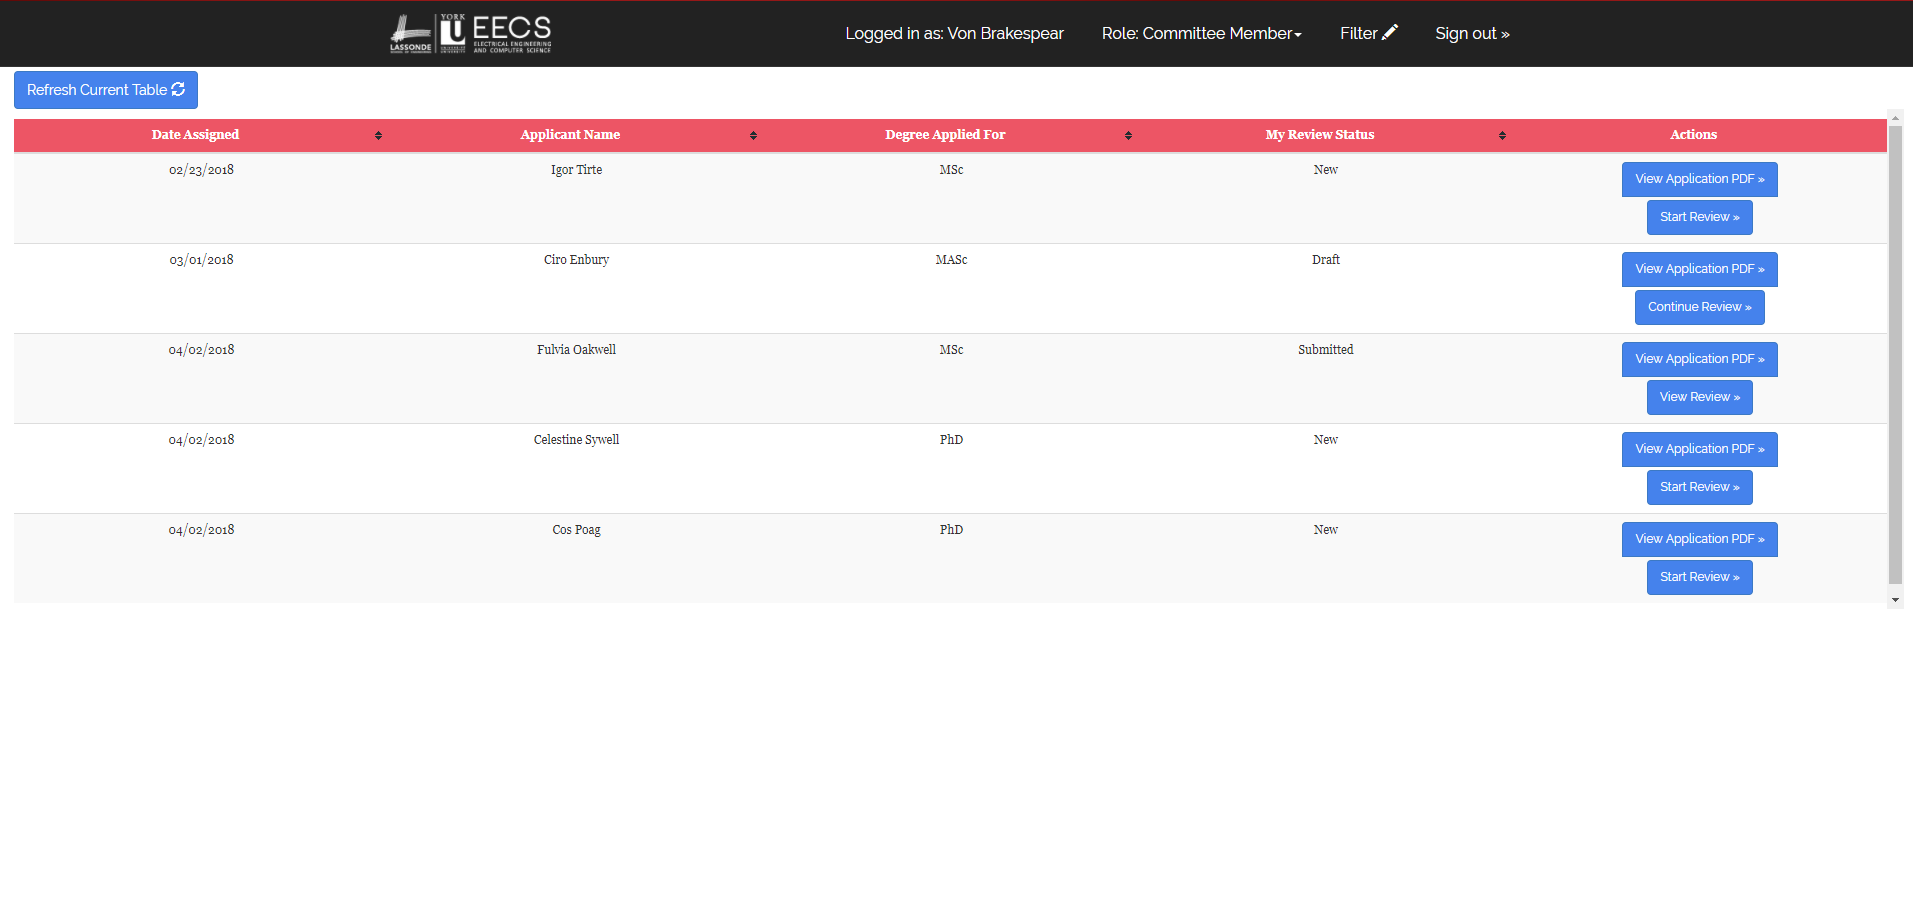
\includegraphics[width=.8\textwidth]{images/default_table.png}
\end{center}
\caption{Committee Member Portal - With Review Applications}
\label{fig:cm_portal}
\end{figure}

\bigskip
\noindent In the actions column, the \emph{View Application PDF} link opens the student application in PDF format uploaded by the system administrator whereas the other Review options open different views of the review form depending on the stage of the review. Refer to Section \ref{sec:reviews} for more information on reviewing an application.

\bigskip
\noindent If there are no reviews assigned to the user, it displays a message to the user.

\begin{figure}[!htb]
\begin{center}
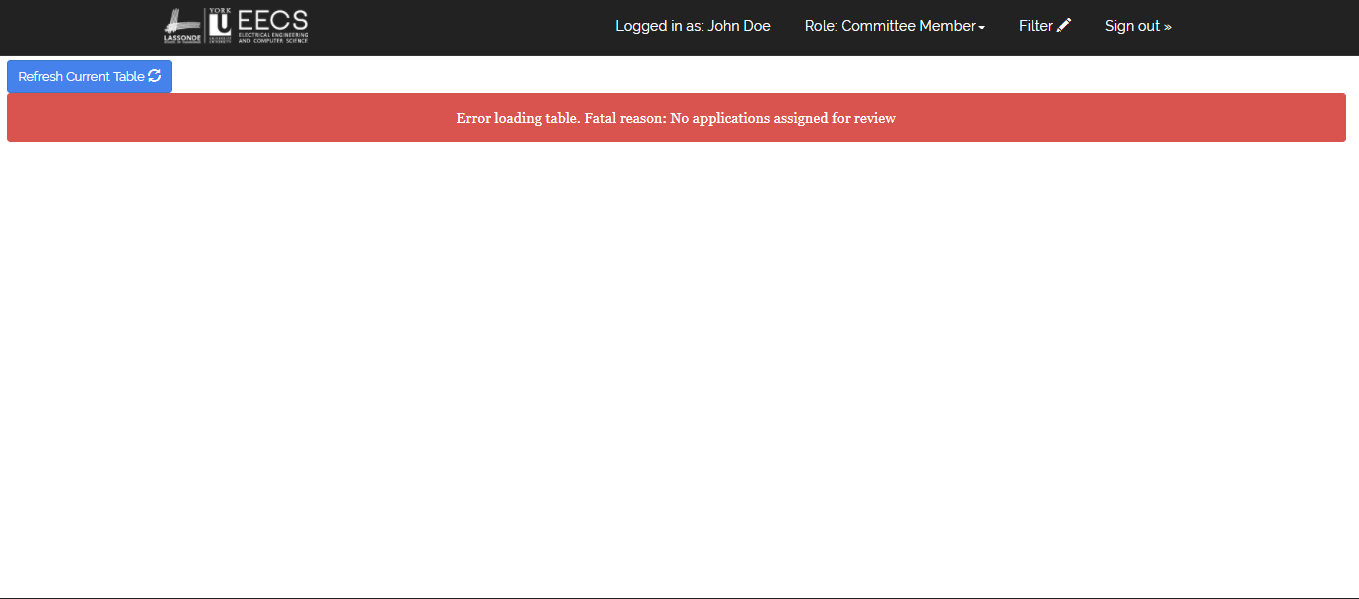
\includegraphics[width=.8\textwidth]{images/err_default.png}
\end{center}
\caption{Committee Member Portal - With No Review Application}
\label{fig:cm_portal_err}
\end{figure}
 
\newpage
\section{Filtering Review Applications}

One of the most powerful tools that Grad Apps 2.0 offers is filtering applications. As a committee member, one can filter past and current assigned review applications. 

\bigskip
\noindent The following image depicts the fields a committee member can apply filtering on as well as the columns they want to see on the resulting table. To open the filter view, simply click on the \emph{pencil} symbol on the top right corner of the portal page.

\begin{figure}[!htb]
\begin{center}
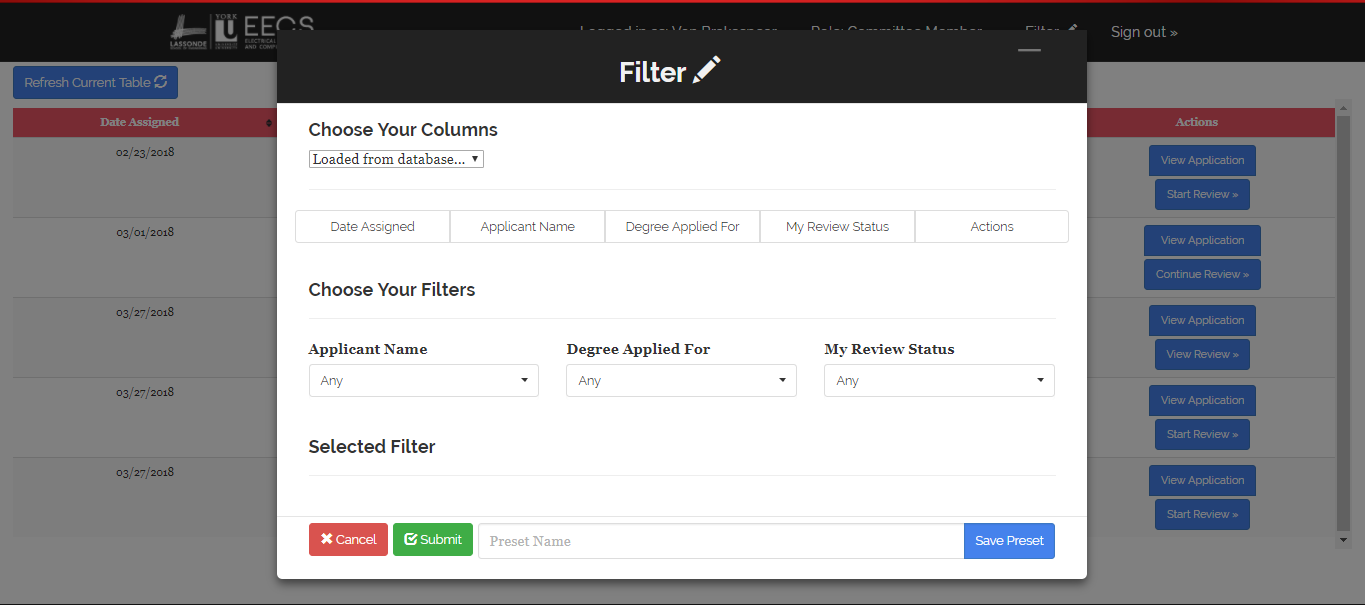
\includegraphics[width=.9\textwidth]{images/default_filter_view.png}
\end{center}
\caption{Filter Selection Modal}
\label{fig:def_filter_modal}
\end{figure}

\newpage
\subsection{Selecting Columns}

After opening the filter view, one can select one or more columns. Selecting a column numbers them in the order they will be displayed after the filter is applied. The following image depicts selecting four columns in order: \emph{Date Assigned, Degree Applied For, My Review Status and Actions}.

\bigskip
\noindent \textbf{Note}: When submitting a filter with no selected columns, all default columns will be used, i.e \emph{Date Assigned, Applicant Name, Degree Applied For, My Review Status and Actions}.

\begin{figure}[!htb]
\begin{center}
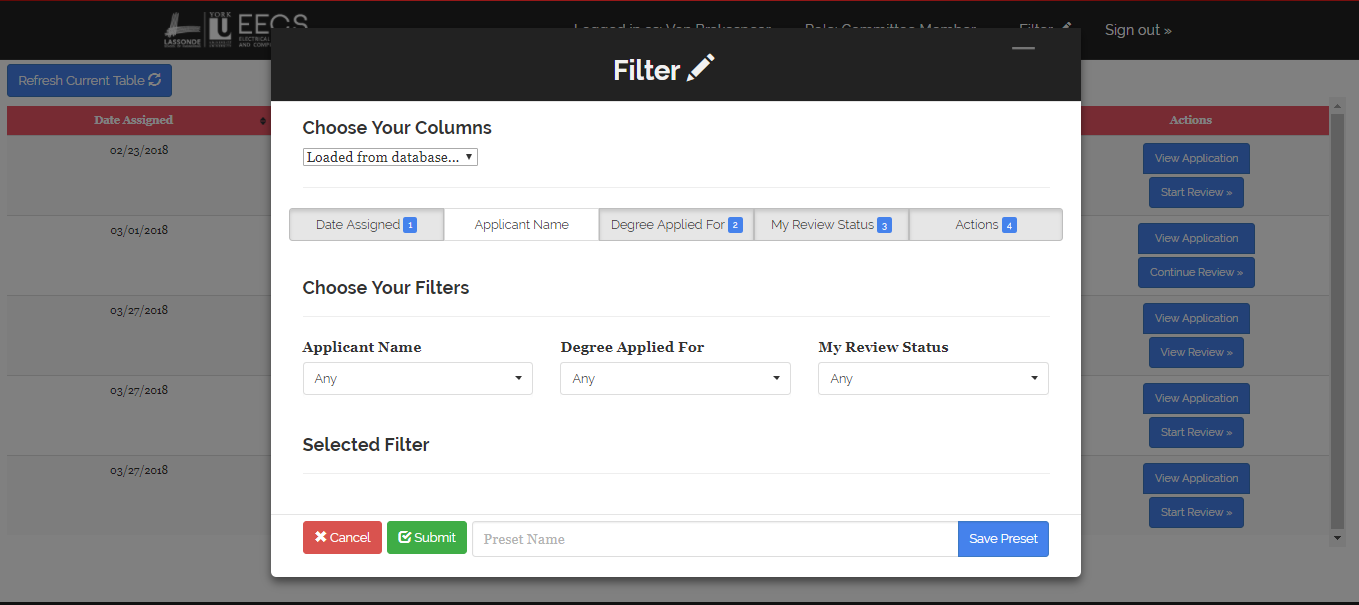
\includegraphics[width=.9\textwidth]{images/selected_col.png}
\end{center}
\caption{Selected Columns for Filter}
\label{fig:fm_selected_col}
\end{figure}

\subsection{Selecting Filter}

After opening the filter view, one can select one or more filters. Selecting a filter can be done only on \emph{Applicant Name}, \emph{Degree Applied For} and \emph{My Review Status} fields. Filtering can be done by selecting values using the selection dropdown which allows live-text searching. The following image depicts selecting a filter for \emph{Degree Applied For} where the Degree is equal to \emph{MSc}.

\bigskip
\noindent \textbf{Note}: When submitting a filter with no selected filters, the default table will be loaded.

\clearpage
\begin{figure}[!htb]
\begin{center}
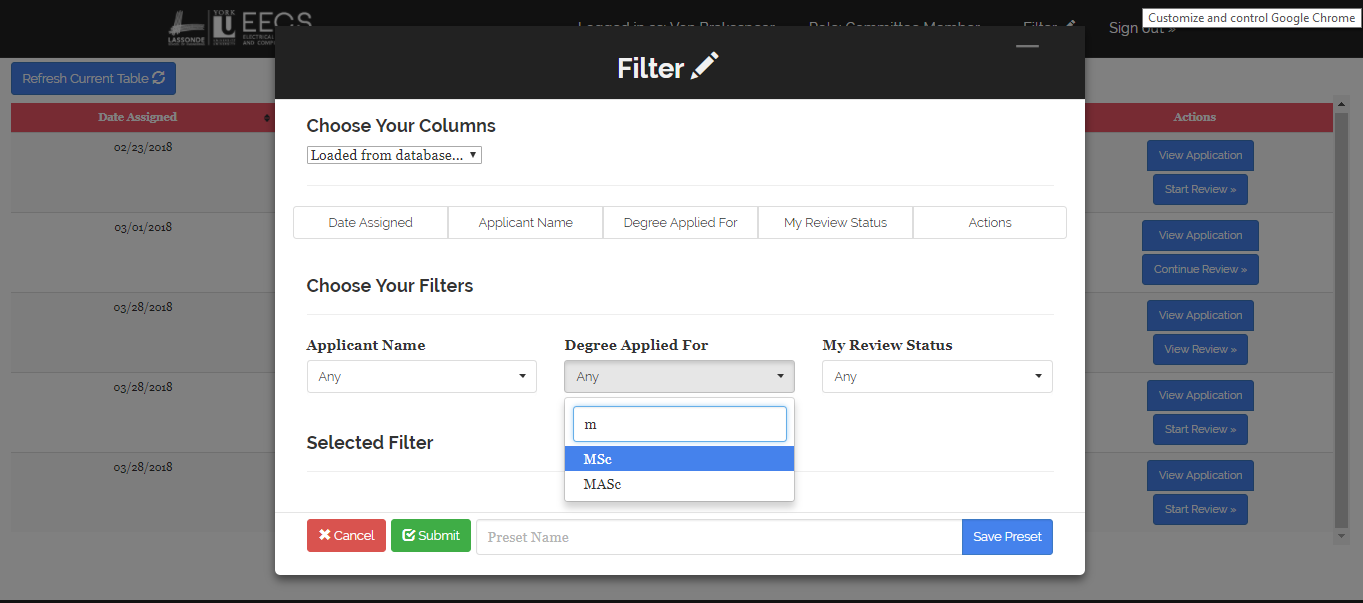
\includegraphics[width=.9\textwidth]{images/selected_filter.png}
\end{center}
\caption{Selected Filter}
\label{fig:fm_selected_filter}
\end{figure}

\bigskip
\noindent Once the user selects a filter, the selected filter text shows the filter chosen. Grad Apps 2.0 only supports \textbf{AND} operand filtering. The image below depicts the selected filter text after selecting a filter for \emph{Degree Applied For} where the Degree is equal to \emph{MSc} and \emph{My Review Status} where review status is equal to \emph{Draft}.

\begin{figure}[!htb]
\begin{center}
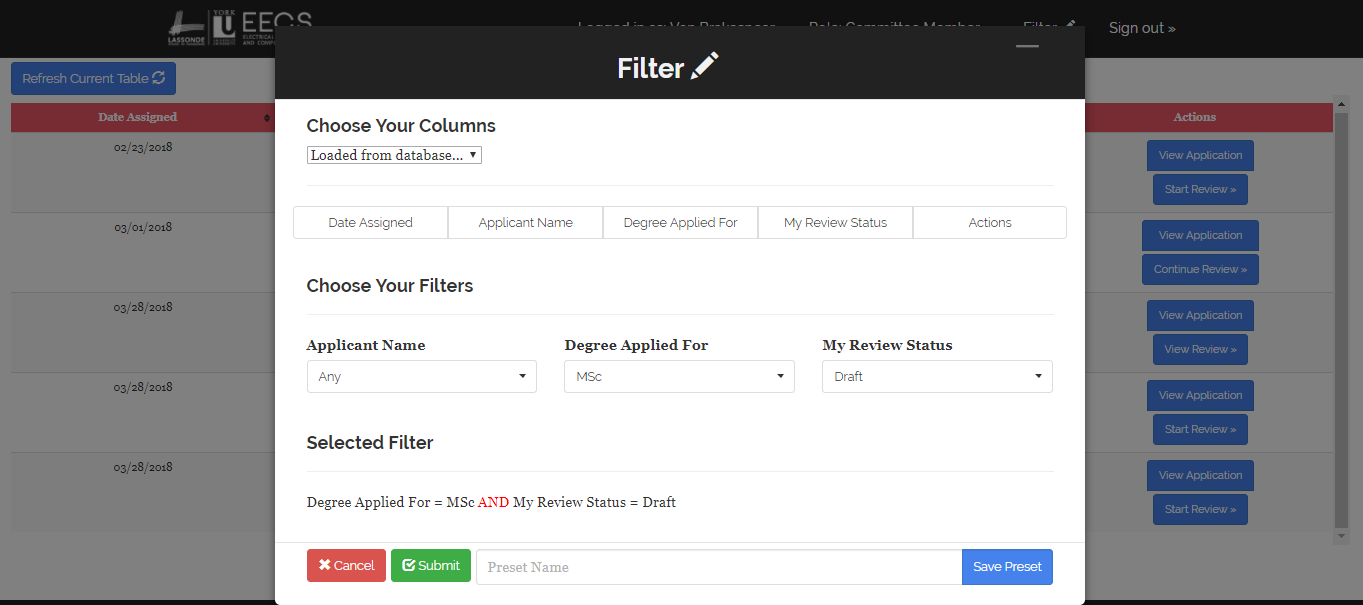
\includegraphics[width=.9\textwidth]{images/selected_filter_text.png}
\end{center}
\caption{Selected Filter Text}
\label{fig:fm_selected_filter_txt}
\end{figure}

\subsection{Filter Presets}
As an end user one can opt to save frequently used filters as presets that will be automatically loaded for the user's login session in that specified role. Saving a filter requires a preset name, the selected rows the user wants to see and the selected filter. 

\bigskip
\noindent The following image depicts on how to save a filter preset:
\begin{figure}[!htb]
\begin{center}
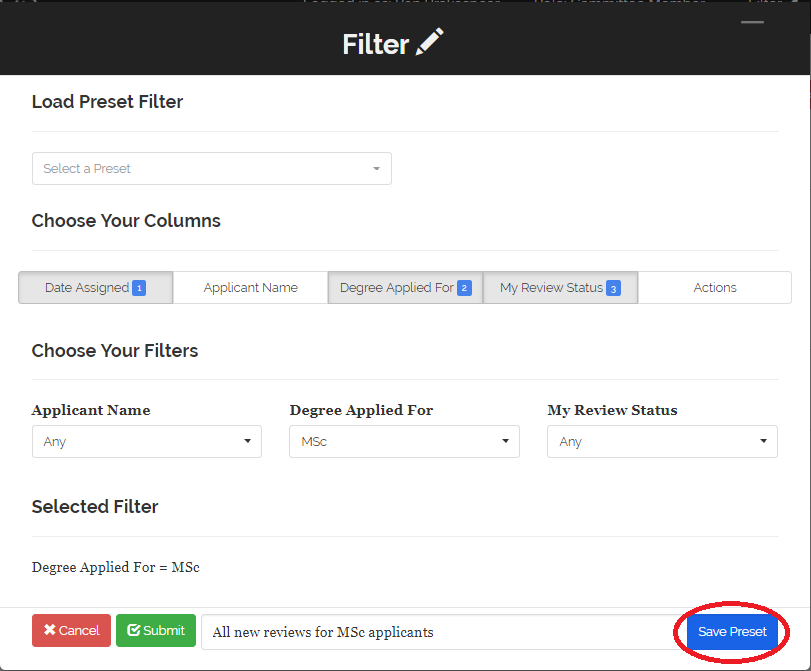
\includegraphics[width=.9\textwidth]{images/saving_preset.png}
\end{center}
\caption{Save a filter preset}
\label{fig:saving_preset}
\end{figure}

\newpage
\bigskip
\noindent Once the user has one or more saved presets, they can opt to load one by simply selecting the preset name from the dropdown. Loading a saved preset will automatically fill the selected columns and the selected filters. The following image depicts on how to load a saved filter preset:

\bigskip
\begin{figure}[!htb]
\begin{center}
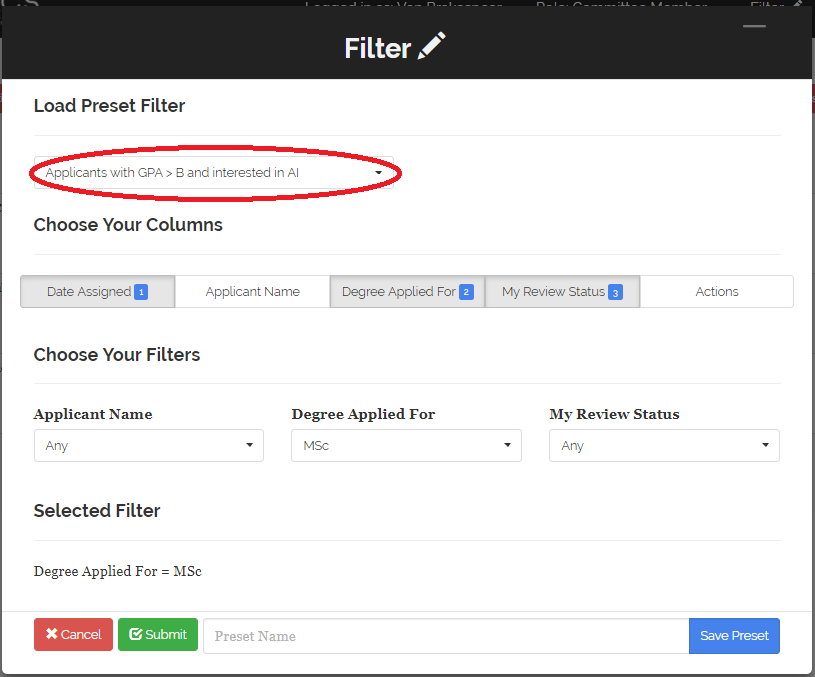
\includegraphics[width=.9\textwidth]{images/load_preset.png}
\end{center}
\caption{Load a saved filter preset}
\label{fig:load_preset}
\end{figure}

\clearpage
\newpage
\subsection{Submitting Filter}

Once the user has selected columns and selected filters, they can submit the filter to get a resulted table back.

\bigskip
\noindent \textbf{Note}: When submitting a filter with no selected columns, all default columns will be used, i.e \emph{Date Assigned, Applicant Name, Degree Applied For, My Review Status and Actions}.

\bigskip
\noindent \textbf{Note}: When submitting a filter with no selected filters, the default table will be loaded.

\bigskip
\noindent The following example filter is used to demonstrate applying a filter and getting the resulted table back:

\bigskip
\noindent \textbf{The columns selected for the filter}:
\begin{enumerate}
\item Date Assigned
\item Degree Applied For
\item My Review Status
\end{enumerate}

\noindent \textbf{The filter selected for}:
\begin{enumerate}
\item Degree Applied For: MSc
\end{enumerate}

\bigskip
\noindent The images below depicts the filter view before applying the filter and the resulting filtered table. The fields used for filtering are also highlighted for emphasizing the filtered fields in the resulting table.

\begin{figure}[!htb]
\begin{center}
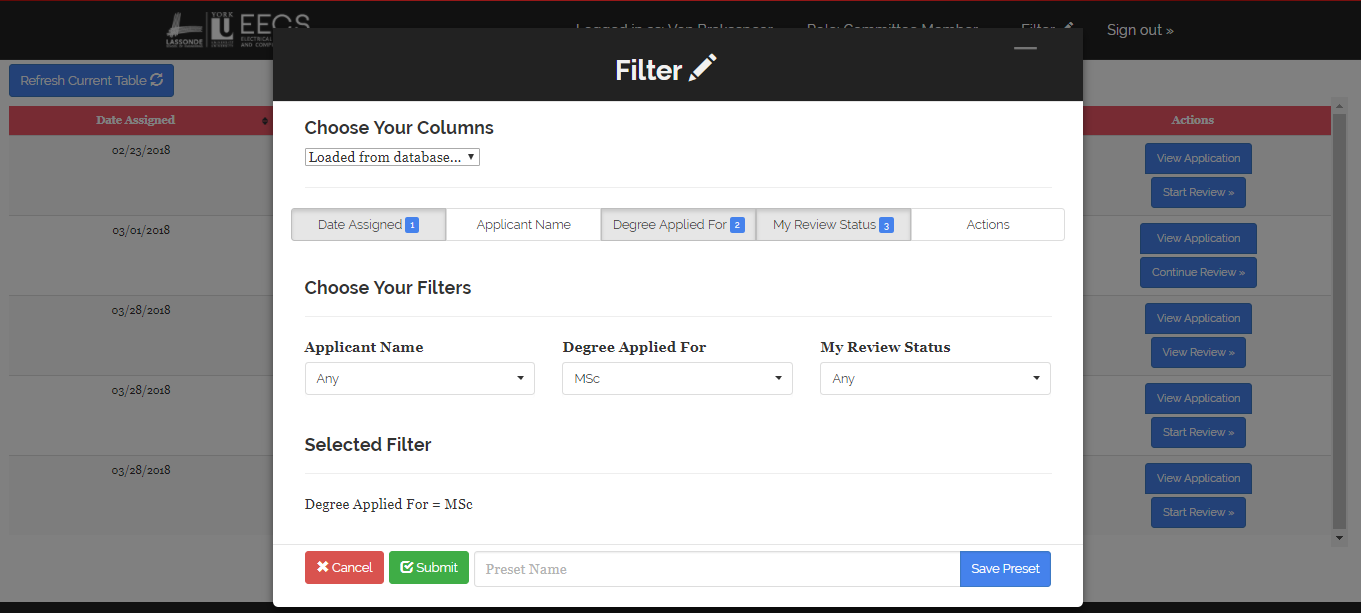
\includegraphics[width=.9\textwidth]{images/example_filter.png}
\end{center}
\caption{Selected Filter Example}
\label{fig:example_filter}
\end{figure}

\begin{figure}[!htb]
\begin{center}
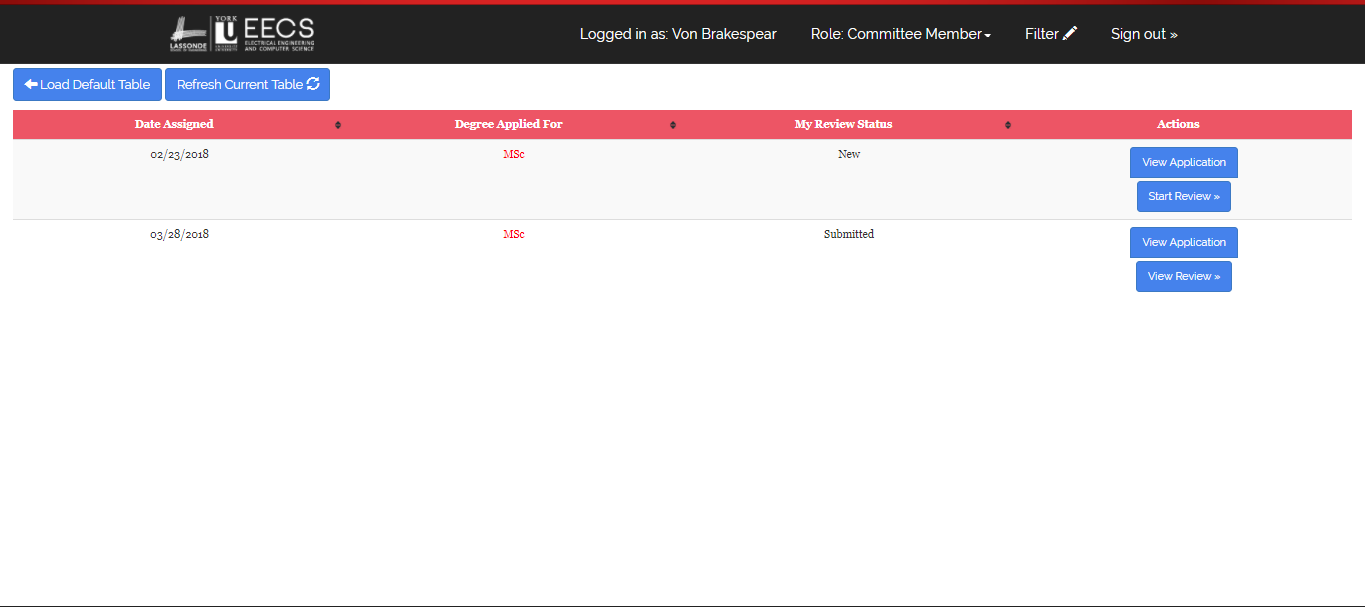
\includegraphics[width=.9\textwidth]{images/example_filter_table.png}
\end{center}
\caption{Resulted Table After Applying Filter}
\label{fig:resulted_table}
\end{figure}

\clearpage
\newpage
\section{Ordering Review Applications}
As a user one can order the fields, either in ascending or descending order, of the table that lists all current and past review applications. The fields that support ordering on review application table are: \emph{Date Assigned}, \emph{Applicant Name}, \emph{Degree Applied For} and \emph{My Review Status}.

\bigskip
\noindent \textbf{Note}: Ordering fields can be done on both filtered and unfiltered review application lists.

\bigskip
\noindent The following images depicts on how to order review applications using the \emph{Date Assigned} field in ascending and descending order.

\begin{figure}[!htb]
\begin{center}
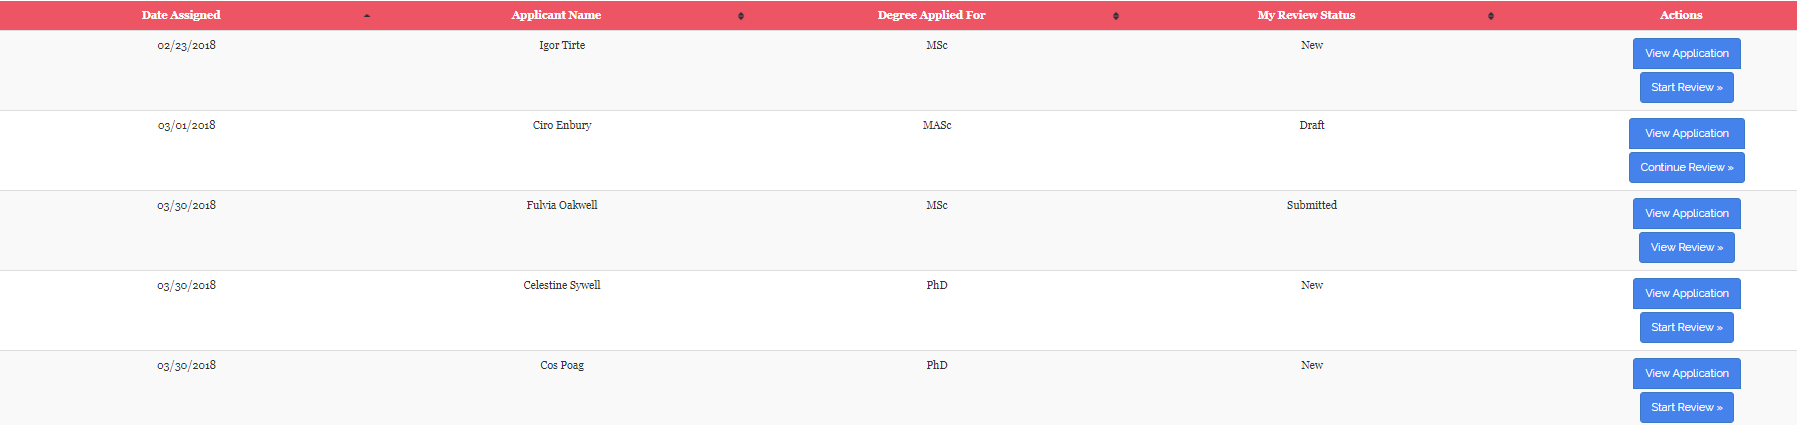
\includegraphics[width=.9\textwidth]{images/order_ascending.png}
\end{center}
\caption{Ascending order of Date Assigned field}
\label{fig:order_ascending}
\end{figure}

\begin{figure}[!htb]
\begin{center}
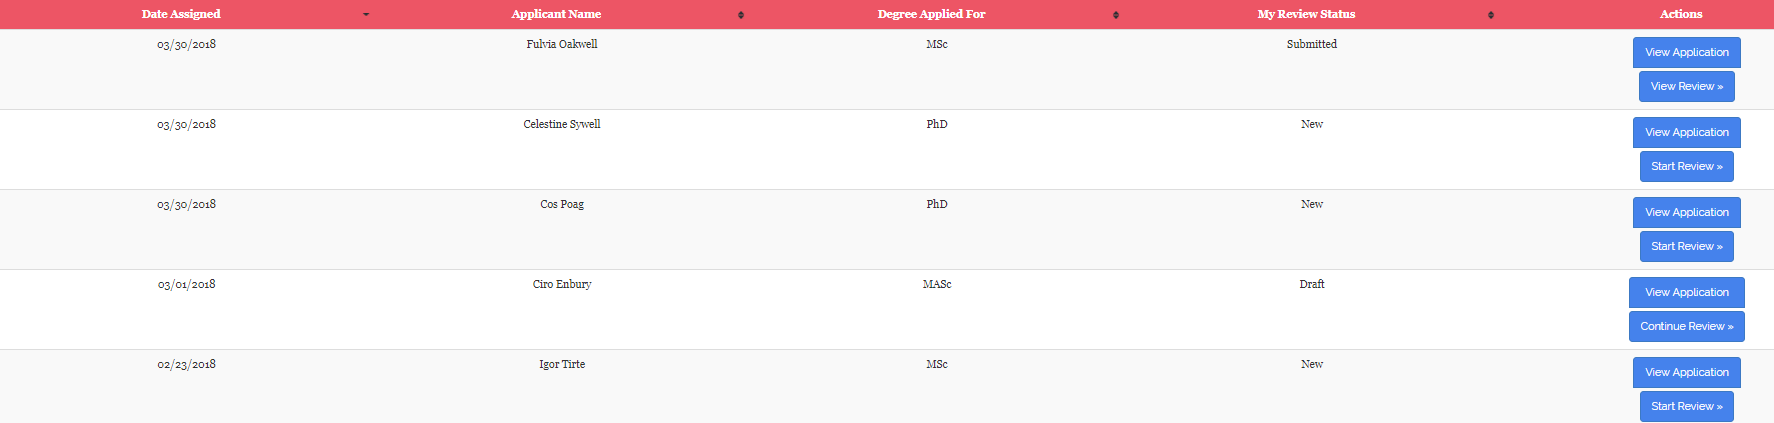
\includegraphics[width=.9\textwidth]{images/order_descending.png}
\end{center}
\caption{Descending order of Date Assigned field}
\label{fig:order_descending}
\end{figure}

\newpage
\bigskip
\noindent \textbf{Note}: One can also apply multiple ordering by holding the SHIFT key on the keyboard and toggling the order. The following images depicts ordering applications with the \emph{Date Assigned} field in ascending order and \emph{Applicant Name} in descending order.

\begin{figure}[!htb]
\begin{center}
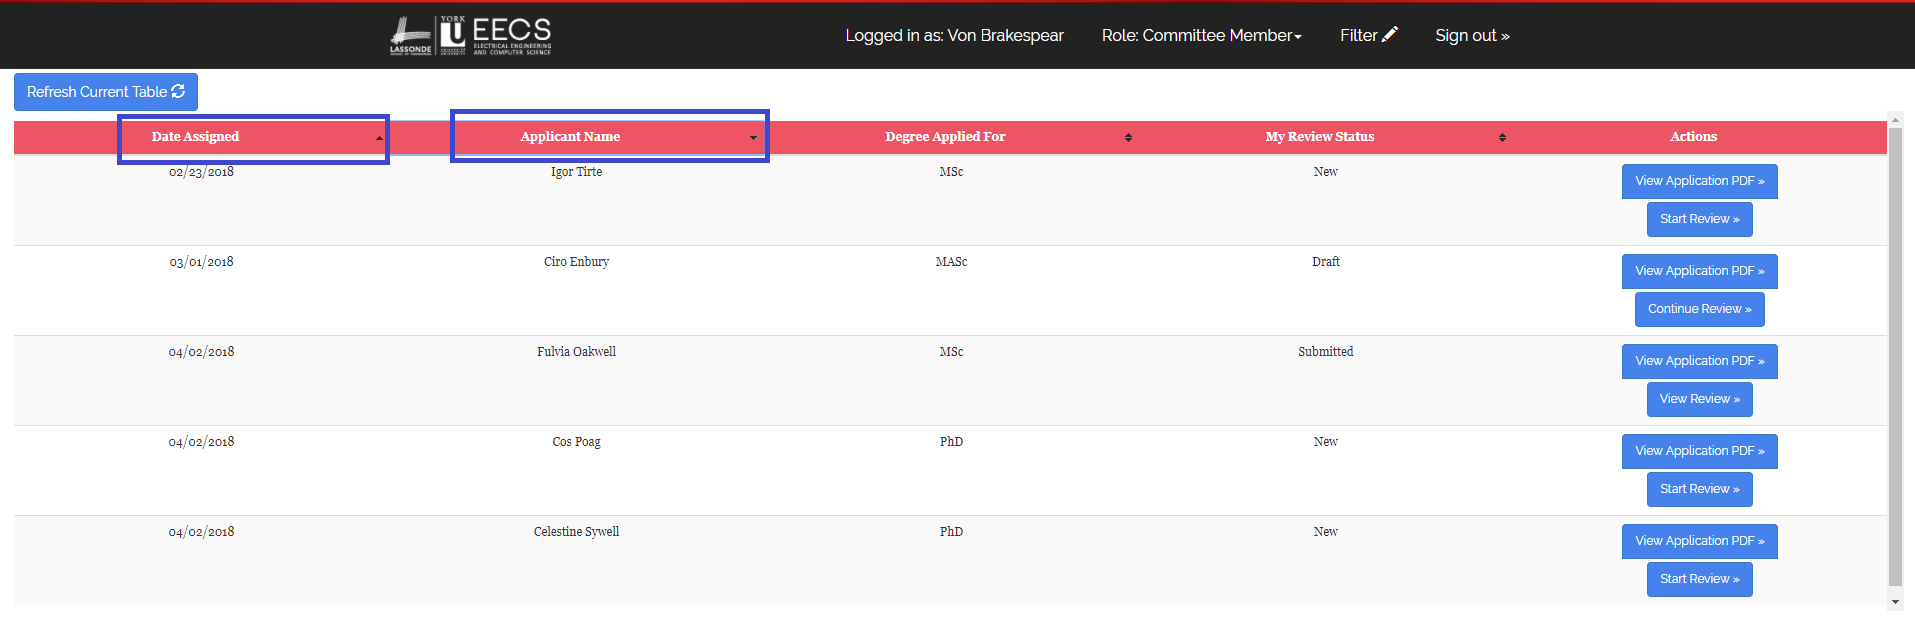
\includegraphics[width=.9\textwidth]{images/multiple_order.png}
\end{center}
\caption{Ordering using multiple fields}
\label{fig:multiple_order}
\end{figure}

\clearpage
\newpage
\section{Reviews} \label{sec:reviews}
As a user one has access to complete application reviews assigned to them by the system administrator. The review process can have \textbf{three} different statuses shown to the user on the default portal:
\begin{itemize}
\item \textbf{New}: A new application has been assigned to the committee member and no changes have been made on the review yet.
\item \textbf{Draft}: A previously saved draft review. A review is considered as a draft when there has been at least one or more changes committed and the user has decided to save the changes.
\item \textbf{Submitted}: A completed review which has been submitted and uploaded to the server. Once a review is submitted, it cannot be undone.
\end{itemize}

\bigskip
\noindent The following list denotes the fields in a review form that is \textbf{not} submitted yet and their requirement status:
\begin{table}[h]
\centering
\begin{tabular}{|c | c |}
	\cline{1-2}
	\textbf{Field Name} & \textbf{Required}\\ \hline
	Institution Name(s) & No \\ \hline
	Institution Assessment(s) & No \\ \hline
	Background Information & No \\ \hline
	Research Experience & No \\ \hline
	Letter of Intent Analysis & No \\ \hline
	Additional Comments & No \\ \hline
	Applicant Rank & Yes \\ \hline
\end{tabular}
\caption {Review Fields}
\label{tbl:review_fields}
\end{table}

\newpage
\bigskip
\noindent The following image depicts the full view of the review form. The \emph{View Application PDF} link opens the student application in PDF version uploaded by the system administrator. 

\begin{figure}[!htb]
\begin{center}
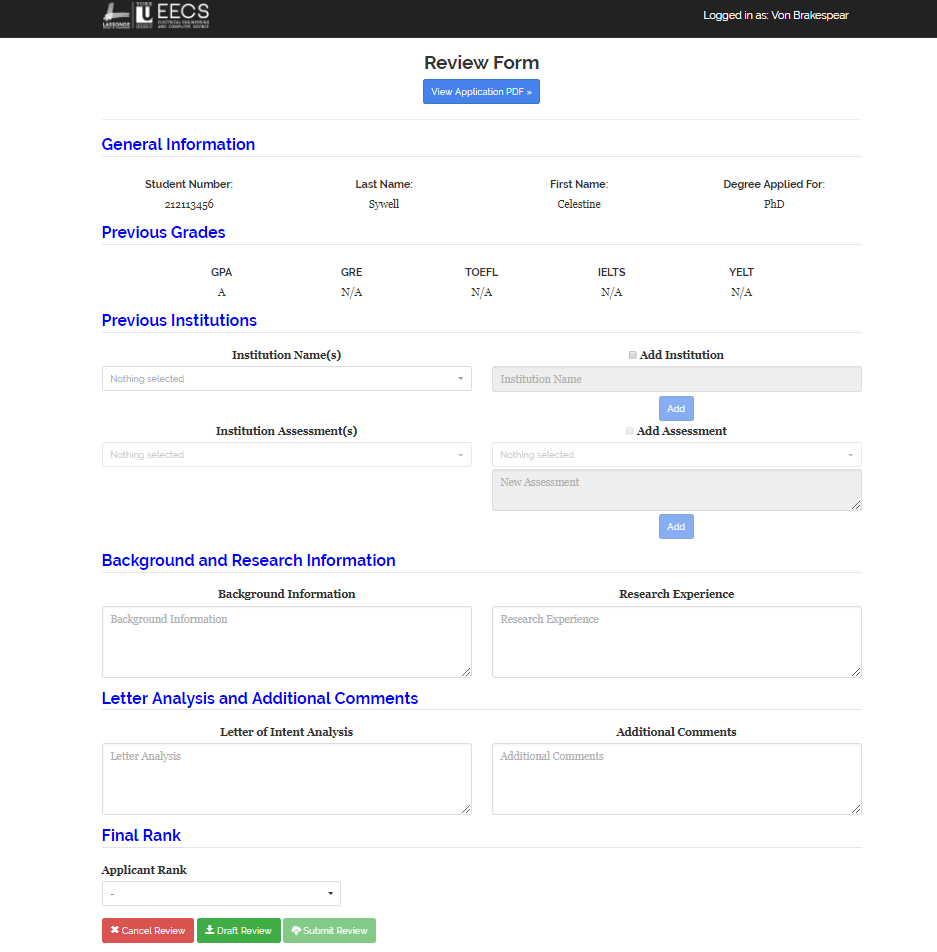
\includegraphics[width=.9\textwidth]{images/review_form.png}
\end{center}
\caption{Full view of the Review Form}
\label{fig:review_form}
\end{figure}

\clearpage
\newpage
\subsection{Opening a new Review}
As a user when a new review is received it will show on the portal. After that the user has the option of opening the review and start completing the form. The action for opening a new review will say \textbf{Start Review}.

\bigskip
\noindent The following image depicts user opening a brand new review.

\begin{figure}[!htb]
\begin{center}
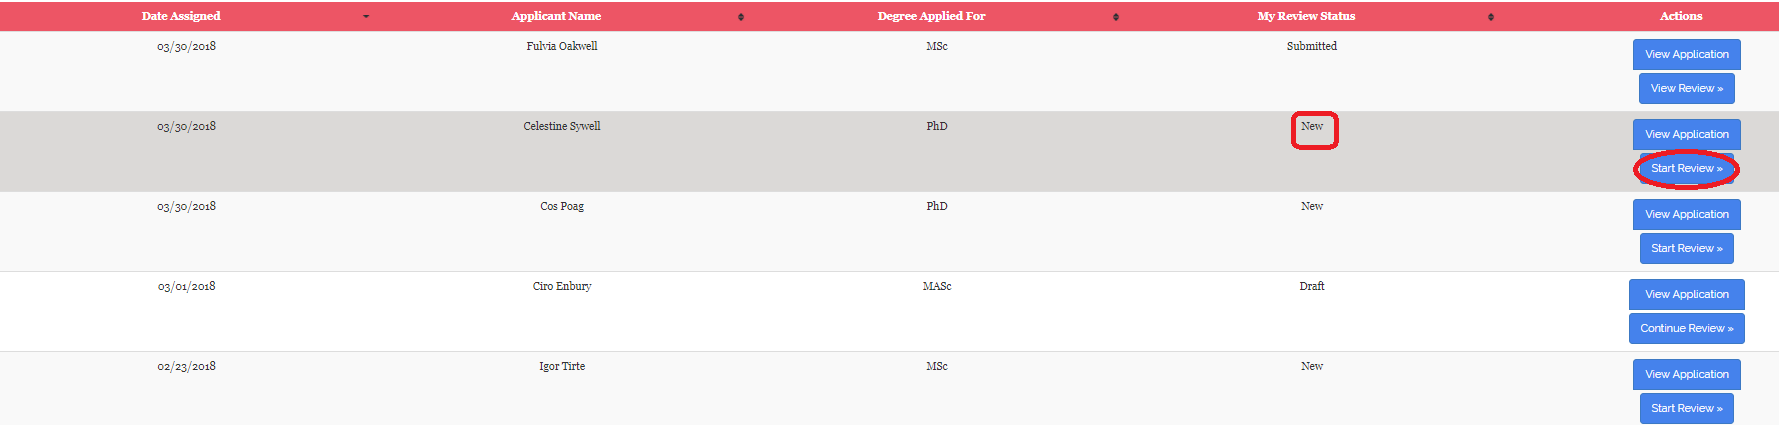
\includegraphics[width=.9\textwidth]{images/opening_new_review.png}
\end{center}
\caption{Opening a brand new review}
\label{fig:opening_new_review}
\end{figure}

\bigskip
\noindent The following image depicts user making no changes to the opened review and exiting out of the review form.

\begin{figure}[!htb]
\begin{center}
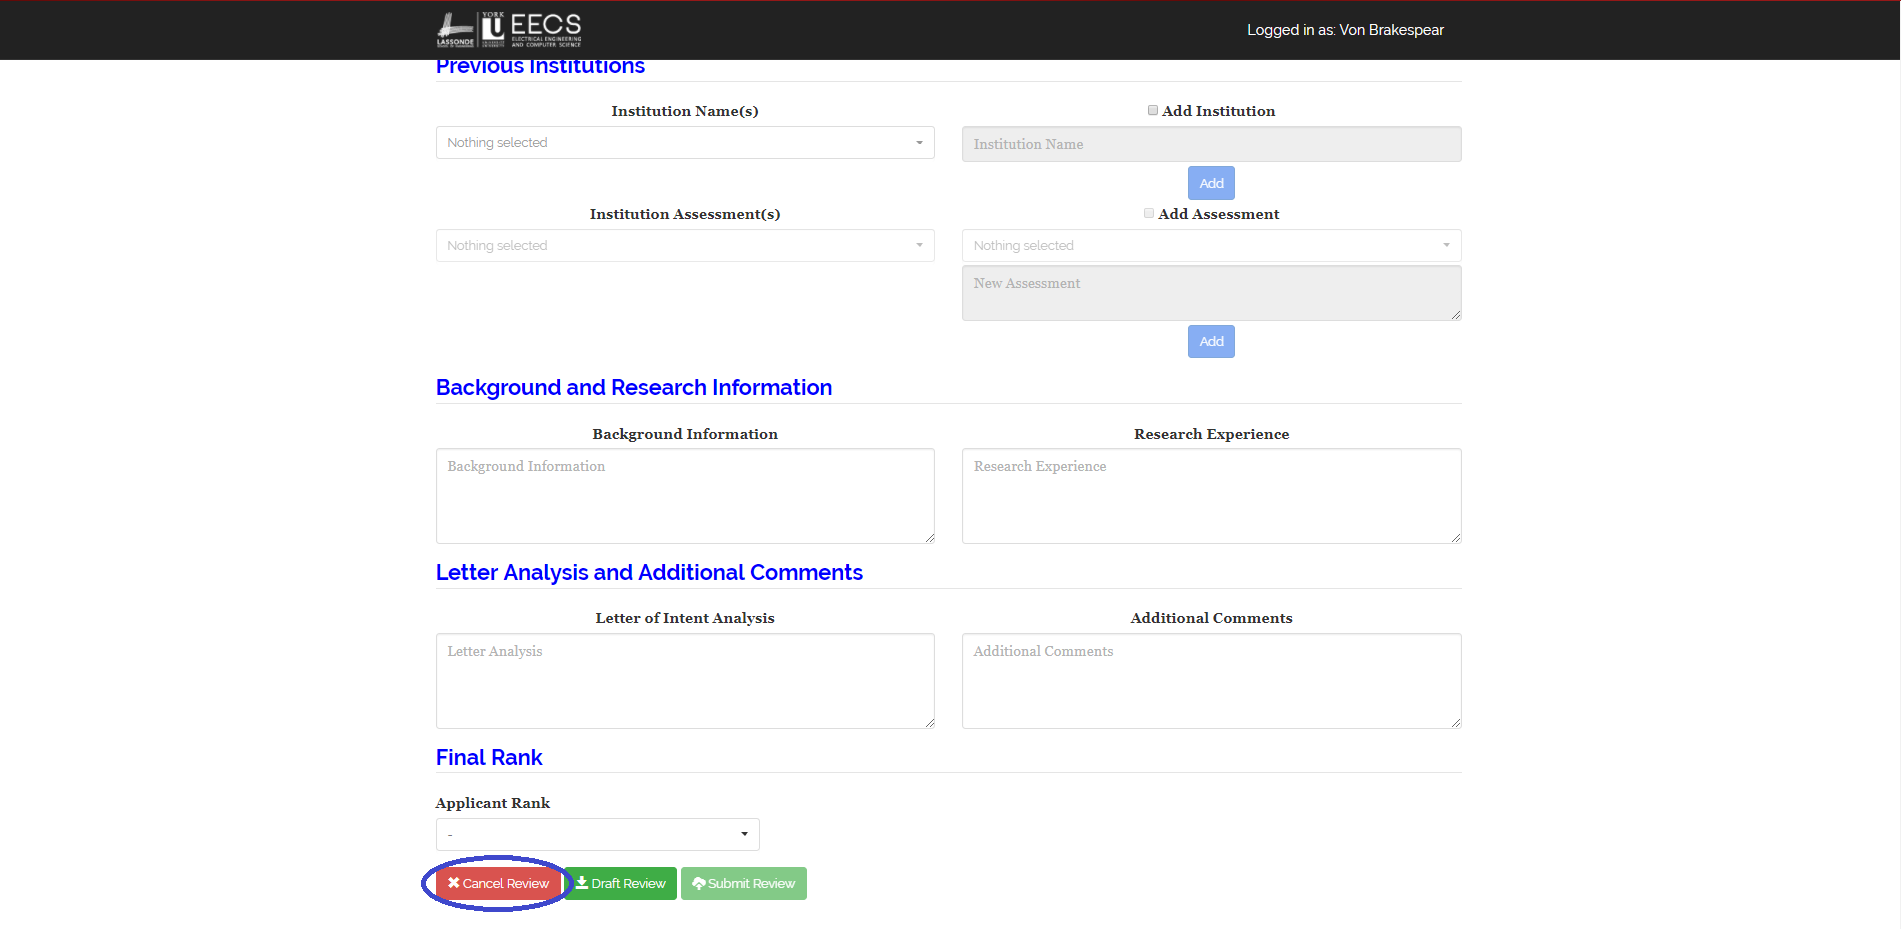
\includegraphics[width=.9\textwidth]{images/new_review_exit_wo_changes.png}
\end{center}
\caption{Exiting out of a brand new review application without changes}
\label{fig:new_review_exit_w/o_changes}
\end{figure}

\subsection{Filling out a Review}
As an end user one has the opportunity to analyse the application assigned for review. Table \ref{tbl:review_fields} outlines the fields in a review application and their required status. The following table specializes Table \ref{tbl:review_fields} and displays the type of input each field takes.

\begin{table}[h]
\centering
\begin{tabular}{|c | c |}
	\cline{1-2}
	\textbf{Field Name} & \textbf{Input Type}\\ \hline
	Institution Name(s) & Multiple Drop-Down \\ \hline
	Institution Assessment(s) & Multiple Drop-Down \\ \hline
	Background Information & Text \\ \hline
	Research Experience & Text \\ \hline
	Letter of Intent Analysis & Text \\ \hline
	Additional Comments & Text \\ \hline
	Applicant Rank & Single Drop-Down \\ \hline
\end{tabular}
\caption {Review Fields Input Type}
\label{tbl:review_fields_input}
\end{table}

\subsubsection{Institution Assessment}
An end user can select one or more institutions the applicant has attended in the past. If the institution does not exist, the user can also add a new institution. Once an institution has been selected, the user can select one or more of the existing institution's assessment and also add a new assessment of their own.

\bigskip
\noindent The following image depicts an user selecting two institutions the applicant has attended and selecting an assessment from each of the institutions.

\begin{figure}[!htb]
\begin{center}
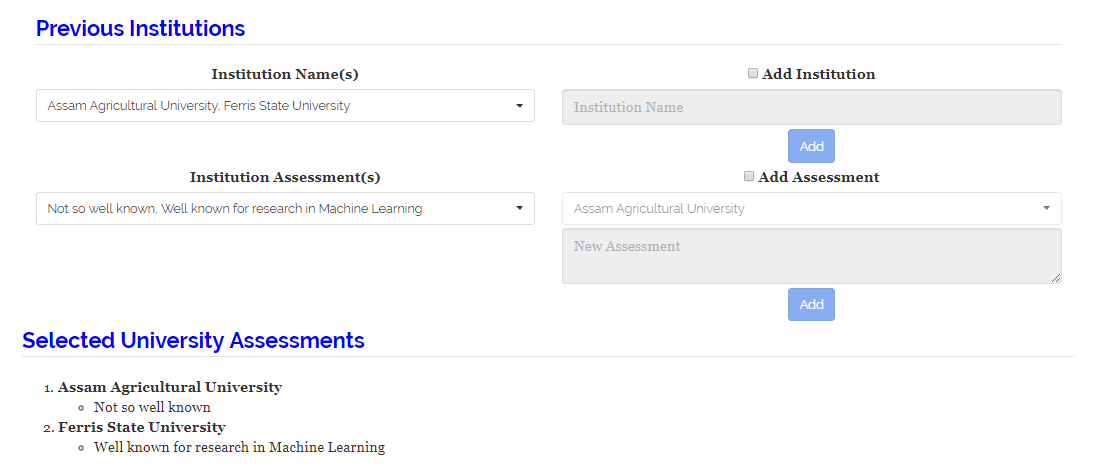
\includegraphics[width=.7\textwidth]{images/uni_assessment.png}
\end{center}
\caption{Institution Assessment View}
\label{fig:uni_assessment}
\end{figure}

\clearpage
\newpage
\subsection{Saving a review as Draft}
As an end user one has the opportunity to save an on-going review as draft for future completion. The use of drafting a review is to save changes to an on-going review so that the user can pick it up and continue some time later.

\bigskip
\noindent The following images depicts a user making changes to an application review and then saving it as a draft. Consequently, the status of the review is changed to \textbf{Draft}. And if the user wants to continue working on the draft sometime later, the action for opening a drafted review will say \textbf{Continue Review}.

\begin{figure}[!htb]
\begin{center}
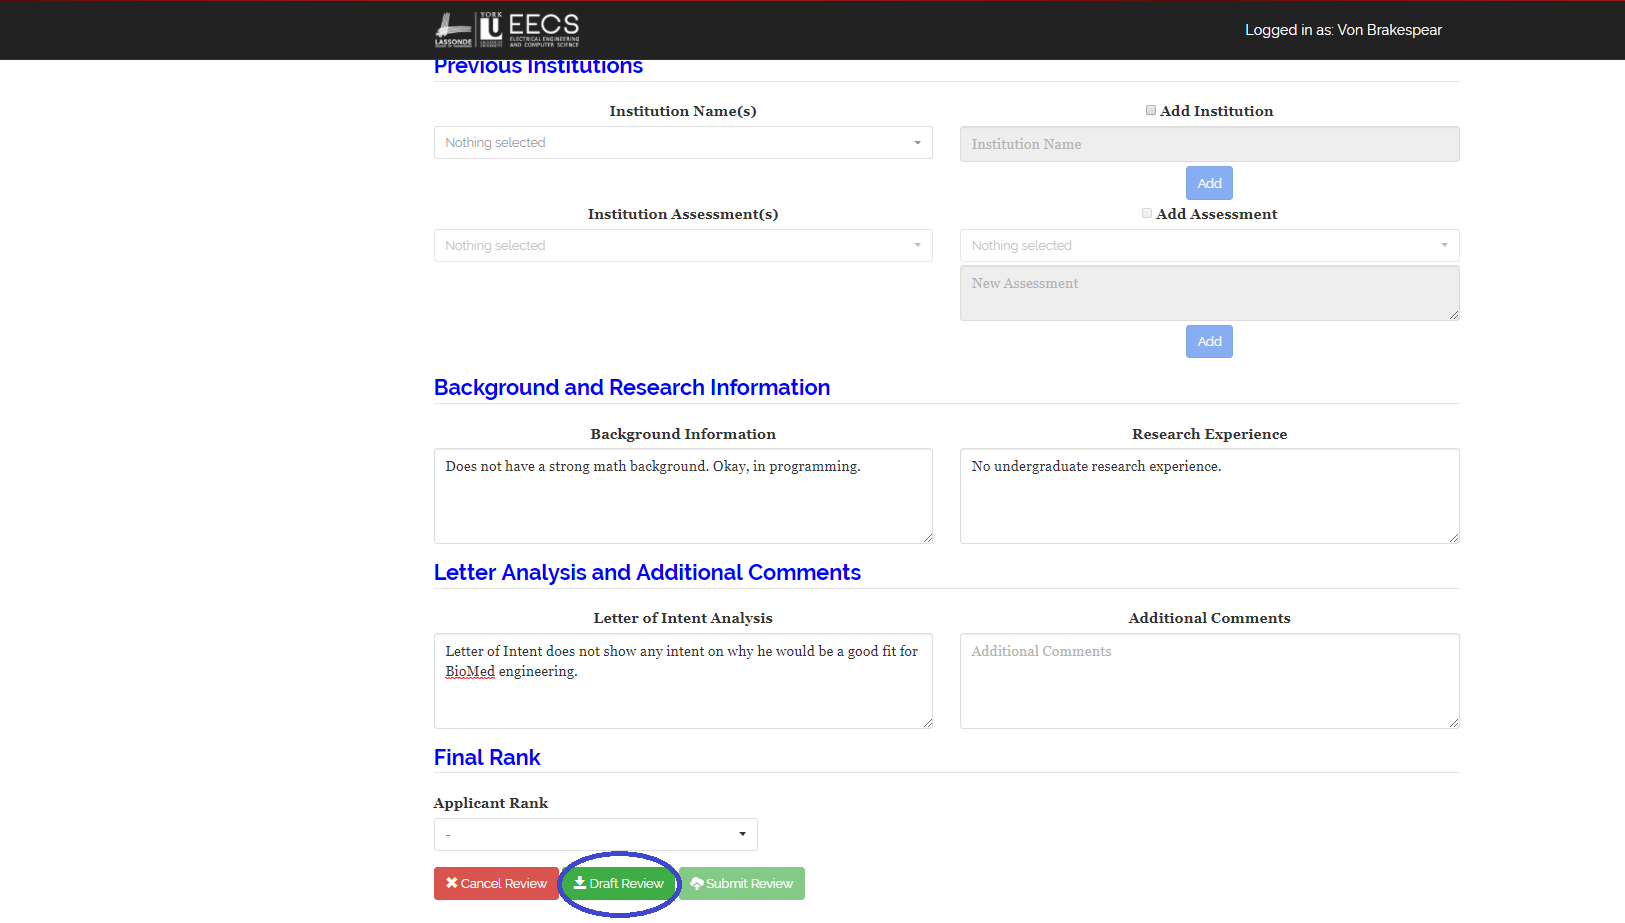
\includegraphics[width=.9\textwidth]{images/save_as_draft_review.png}
\end{center}
\caption{Save a review as draft}
\label{fig:save_as_draft_review}
\end{figure}

\begin{figure}[!htb]
\begin{center}
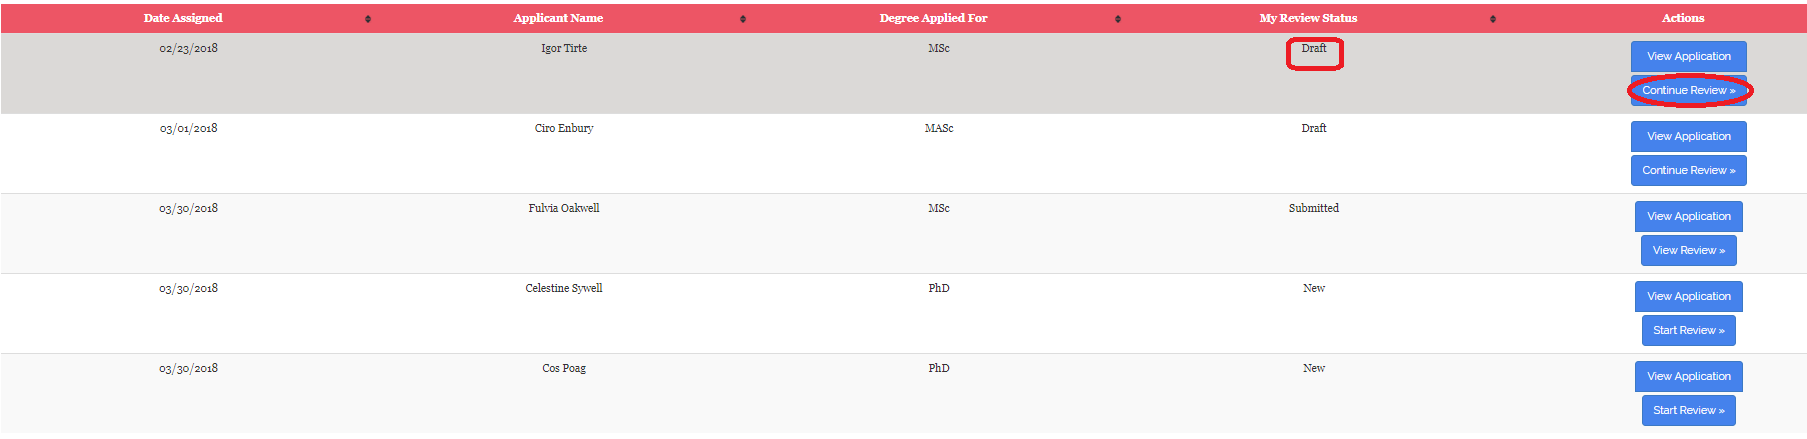
\includegraphics[width=.9\textwidth]{images/drafted_review.png}
\end{center}
\caption{Drafted Review View}
\label{fig:drafted_review}
\end{figure}

\subsection{Submitting a Review}
Once a review is completed, the user can submit the review. If the correct number of reviews for an application has been submitted, the application will be automatically available for selection to the members of EECS Graduate Program. The only required field needed for submitting a review is the final application rank that is to be decided by the admission committee member upon analysing the application.

\bigskip
\noindent The following image depicts an end user submitting a review. 

\begin{figure}[!htb]
\begin{center}
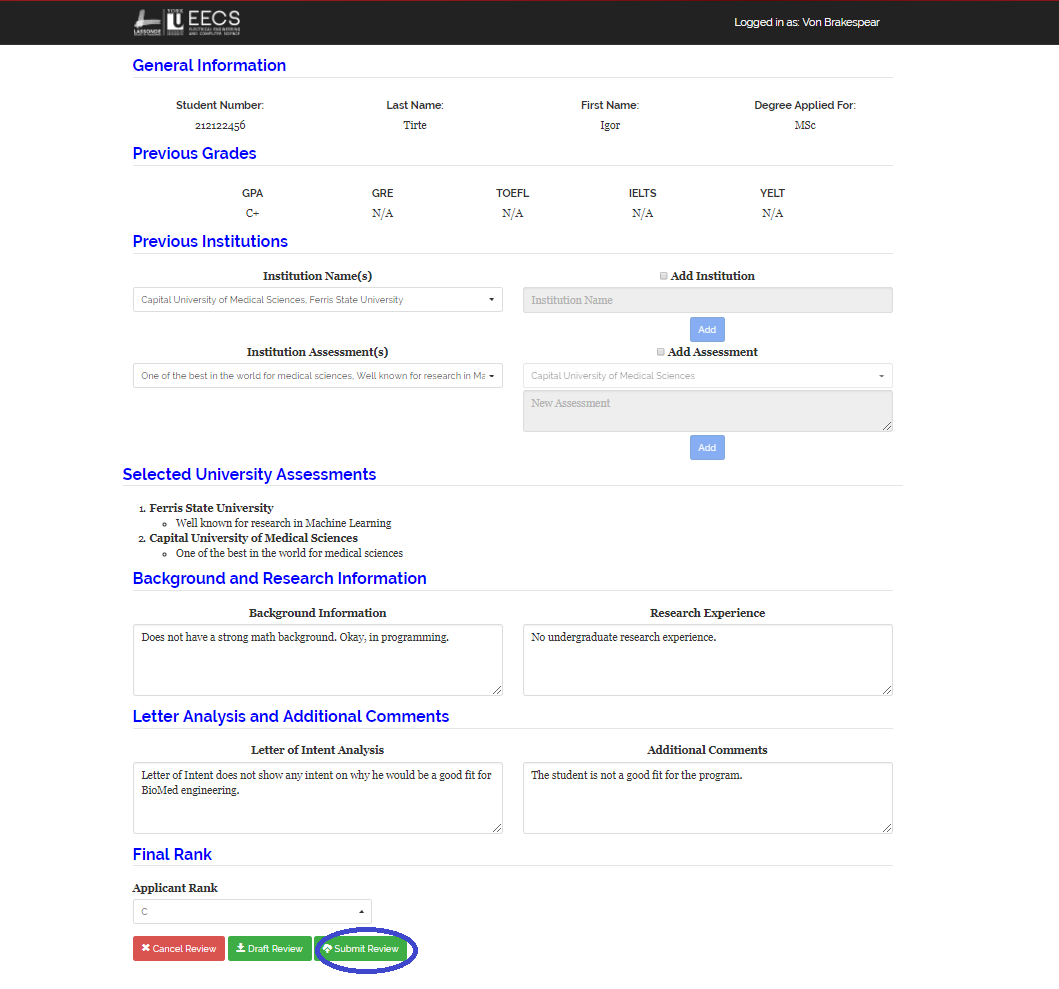
\includegraphics[width=.9\textwidth]{images/submit_review.png}
\end{center}
\caption{Submit a Review}
\label{fig:submit_review}
\end{figure}

\bigskip
\noindent Once the review is submitted, it will show up on the user dashboard with status as \textbf{Submitted}. The user action to view a submitted review will say \textbf{View Review}. Submitted reviews are only viewable as a plain text application form. The following images depicts viewing a submitted review.

\begin{figure}[!htb]
\begin{center}
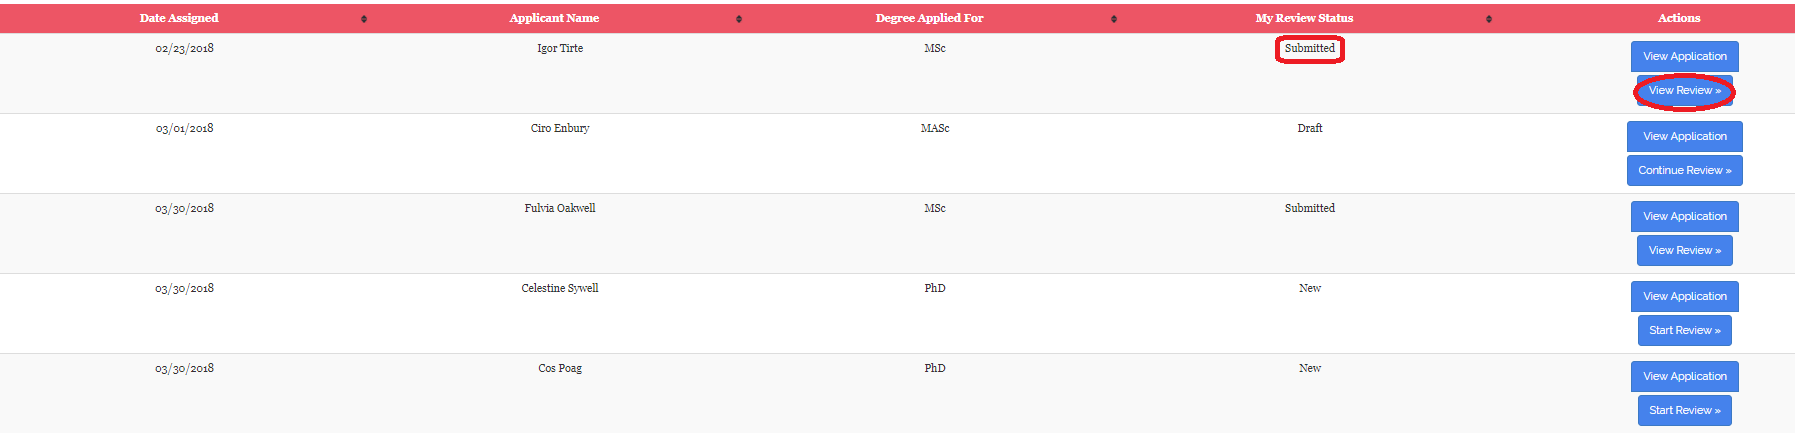
\includegraphics[width=.9\textwidth]{images/submitted_review.png}
\end{center}
\caption{Submitted Review View}
\label{fig:submitted_review}
\end{figure}

\begin{figure}[!htb]
\begin{center}
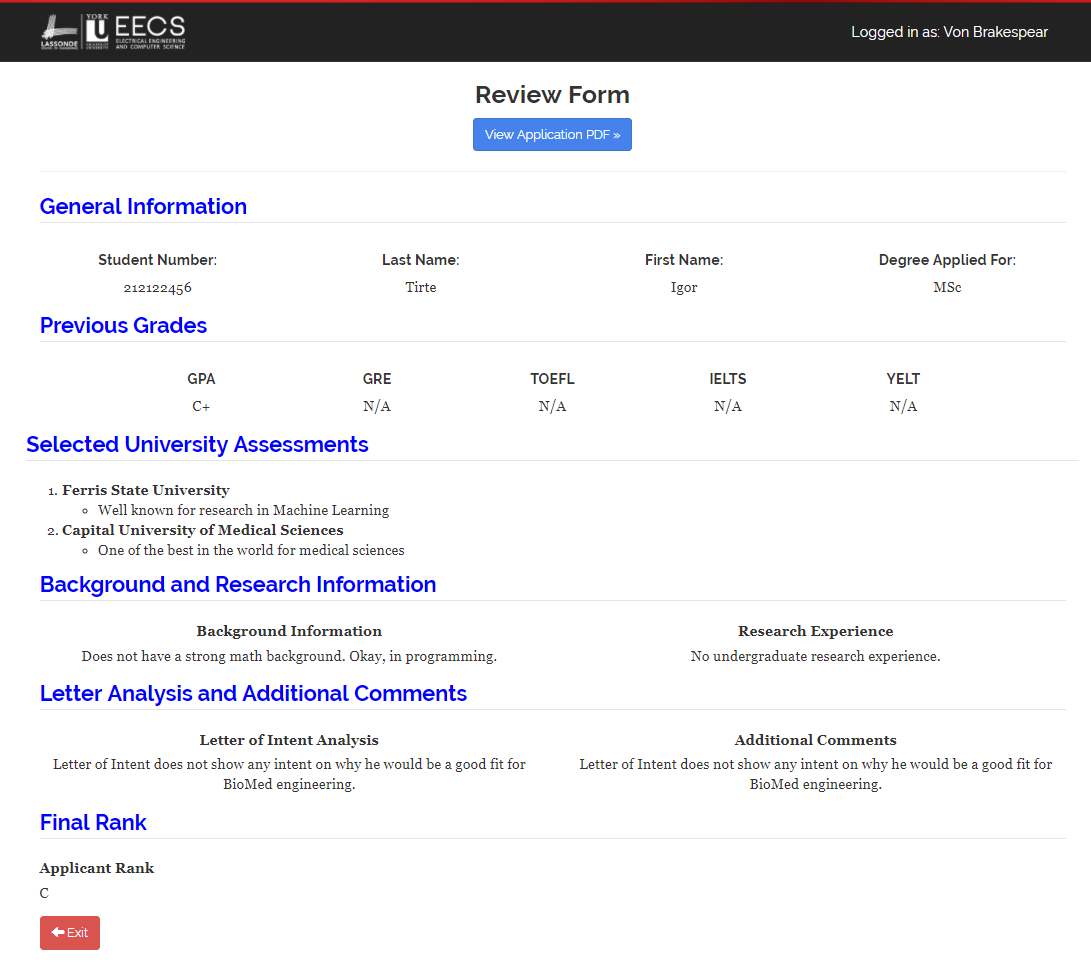
\includegraphics[width=.7\textwidth]{images/submit_review_view.png}
\end{center}
\caption{Submitted Review View}
\label{fig:submit_review_view}
\end{figure}

\end{document}